\documentclass[
11pt, % The default document font size, options: 10pt, 11pt, 12pt
%codirector, % Uncomment to add a codirector to the title page
]{charter} 




% El títulos de la memoria, se usa en la carátula y se puede usar el cualquier lugar del documento con el comando \ttitle
\titulo{Controlador CAN de Servomotores} 

% Nombre del posgrado, se usa en la carátula y se puede usar el cualquier lugar del documento con el comando \degreename
\posgrado{Carrera de Especialización en Sistemas Embebidos} 
%\posgrado{Carrera de Especialización en Internet de las Cosas} 
%\posgrado{Carrera de Especialización en Intelegencia Artificial}
%\posgrado{Maestría en Sistemas Embebidos} 
%\posgrado{Maestría en Internet de las cosas}

% Tu nombre, se puede usar el cualquier lugar del documento con el comando \authorname
\autor{Alejandro Virgillo} 

% El nombre del director y co-director, se puede usar el cualquier lugar del documento con el comando \supname y \cosupname y \pertesupname y \pertecosupname
\director{Gabriel Gavinowich}
\pertenenciaDirector{FIUBA} 

\codirector{} % para que aparezca en la portada se debe descomentar la opción codirector en el documentclass
\pertenenciaCoDirector{}

% Nombre del cliente, quien va a aprobar los resultados del proyecto, se puede usar con el comando \clientename y \empclientename
\cliente{Alejandro Virgillo}
\empresaCliente{A3 Engineering}

% Nombre y pertenencia de los jurados, se pueden usar el cualquier lugar del documento con el comando \jurunoname, \jurdosname y \jurtresname y \perteunoname, \pertedosname y \pertetresname.
\juradoUno{Nombre y Apellido (1)}
\pertenenciaJurUno{pertenencia (1)} 
\juradoDos{Nombre y Apellido (2)}
\pertenenciaJurDos{pertenencia (2)}
\juradoTres{Nombre y Apellido (3)}
\pertenenciaJurTres{pertenencia (3)}
 
\fechaINICIO{21 de octubre de 2021}		%Fecha de inicio de la cursada de GdP \fechaInicioName
\fechaFINALPlan{9 de diciembre de 2021} 	%Fecha de final de cursada de GdP
\fechaFINALTrabajo{9 de octubre de 2022}	%Fecha de defensa pública del trabajo final


\begin{document}

\maketitle
\thispagestyle{empty}
\pagebreak


\thispagestyle{empty}
{\setlength{\parskip}{0pt}
\tableofcontents{}
}
\pagebreak


\section*{Registros de cambios}
\label{sec:registro}


\begin{table}[ht]
\label{tab:registro}
\centering
\begin{tabularx}{\linewidth}{@{}|c|X|c|@{}}
\hline
\rowcolor[HTML]{C0C0C0} 
Revisión & \multicolumn{1}{c|}{\cellcolor[HTML]{C0C0C0}Detalles de los cambios realizados} & Fecha      \\ \hline
0      & Creación del documento                                 &\fechaInicioName \\ \hline
1      & Se completa hasta el punto 5 inclusive                 & 30 de octubre de 2021 \\ \hline
2      & Se completa hasta el punto 9 inclusive
& 7 de noviembre de 2021 \\ \hline
3      & Se completa hasta el punto 11 inclusive                & 16 de noviembre de 2021 \\ \hline
%4      & Se completa el plan	                                 & dd/mm/aaaa \\ \hline
\end{tabularx}
\end{table}

\pagebreak



\section*{Acta de constitución del proyecto}
\label{sec:acta}

\begin{flushright}
Buenos Aires, \fechaInicioName
\end{flushright}

\vspace{2cm}

Por medio de la presente se acuerda con el Ing. \authorname\hspace{1px} que su Trabajo Final de la \degreename\hspace{1px} se titulará ``\ttitle'', consistirá esencialmente en la implementación de una interfaz que permita configurar y relevar información de servomotores conectados a través de una red CAN, y tendrá un presupuesto preliminar estimado de 600 hs de trabajo y U\$1000, con fecha de inicio \fechaInicioName\hspace{1px} y fecha de presentación pública \fechaFinalName.

Se adjunta a esta acta la planificación inicial.

\vfill

% Esta parte se construye sola con la información que hayan cargado en el preámbulo del documento y no debe modificarla
\begin{table}[ht]
\centering
\begin{tabular}{ccc}
\begin{tabular}[c]{@{}c@{}}Ariel Lutenberg \\ Director posgrado FIUBA\end{tabular} & \hspace{2cm} & \begin{tabular}[c]{@{}c@{}}\clientename \\ \empclientename \end{tabular} \vspace{2.5cm} \\ 
\multicolumn{3}{c}{\begin{tabular}[c]{@{}c@{}} \supname \\ Director del Trabajo Final\end{tabular}} \vspace{2.5cm} \\
%\begin{tabular}[c]{@{}c@{}}\jurunoname \\ Jurado del Trabajo Final\end{tabular}     &  & \begin{tabular}[c]{@{}c@{}}\jurdosname\\ Jurado del Trabajo Final\end{tabular}  \vspace{2.5cm}  \\
%\multicolumn{3}{c}{\begin{tabular}[c]{@{}c@{}} \jurtresname\\ Jurado del Trabajo Final\end{tabular}} \vspace{.5cm}                                                                     
\end{tabular}
\end{table}




\section{1. Descripción técnica-conceptual del proyecto a realizar}
\label{sec:descripcion}

El proyecto busca obtener un dispositivo que permita programar y supervisar servomotores conectados dentro de una red CAN (\textit{Controller Area Network}), así como relevar información de estos. El resultado debe ser de carácter industrial, por lo que se prioriza su robustez para poder operar en planta y debe contar con una interfaz de usuario.

La organización \empclientename{} desarrolló un sistema embebido, llamado SN-17, capaz de controlar la posición, velocidad, aceleración y torque a motores del tipo paso a paso, también conocidos como \textit{steppers}. Actualmente, varios de estos motores, junto con las placas controladoras mencionadas, se encuentran en funcionamiento en la planta de la empresa Cambre, realizando diversos tipos de actuaciones mecánicas en líneas de manufactura.

El sistema SN-17 cuenta con un problema, que es la dificultad para alterar, de forma cómoda, el funcionamiento de los motores. El firmware debe ser modificado cada vez que se quiera realizar un cambio de este estilo, lo cual limita la operabilidad. 

Dentro de este contexto es que se propone el actual proyecto. Se buscará lograr una interfaz que permita a un usuario con poco entrenamiento conectarse con los motores y modificar los parámetros de funcionamiento. Para ello, se establecerá comunicación a través de una red CAN, aprovechando que el sistema SN-17 cuenta con un puerto para este protocolo. Es necesario, entonces, diseñar un sistema de mensajeria que haga que los dispositivos puedan enviar información dentro de la red, y una interfaz gráfica que permita a usuarios realizar cambios.

También se propone que el dispositivo actue como supervisor, una vez que los motores estén en funcionamiento. Como en la mayoría de procesos industriales suelen emplearse controladores PLC (\textit{Programmable Logic Controller}), es necesario que la solución buscada pueda interactuar con estos.

En la Figura 1 se muestra, a modo de ejemplo, un diagrama en bloques del sistema. El proyecto abarca el diseño y fabricación de la parte que aparece denominada como controlador y su interacción con los demás bloques. También notar que en el bus CAN pueden haber conectados más de 1 servomotor. Cada uno de estos tendrá una de las placas controladoras descriptas previamente.

\begin{figure}[htpb]
\centering 
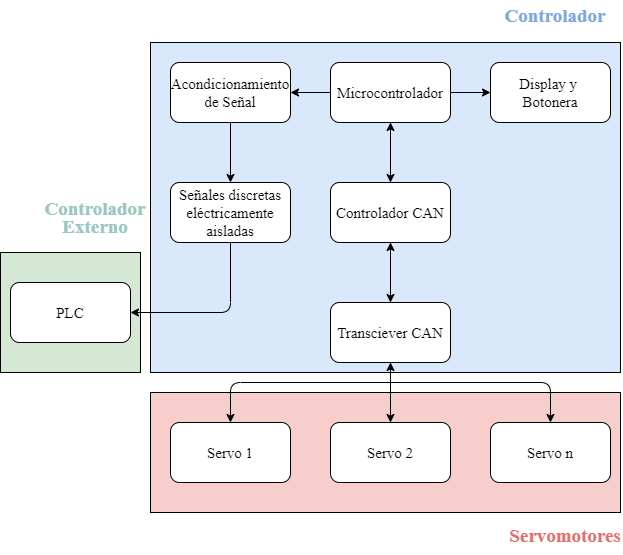
\includegraphics[width=.8\textwidth]{./Figuras/CAN_Servo_controller.png}
\caption{Diagrama en bloques del sistema}
\label{fig:diagBloques}
\end{figure}


\section{2. Identificación y análisis de los interesados}
\label{sec:interesados}

\begin{table}[ht]
%\caption{Identificación de los interesados}
%\label{tab:interesados}
\begin{tabularx}{\linewidth}{@{}|l|X|X|l|@{}}
\hline
\rowcolor[HTML]{C0C0C0} 
Rol           & Nombre y Apellido & Organización 	& Puesto 	\\ \hline
Auspiciante   & \clientename      & \empclientename	&       Líder de proyecto 	\\ \hline
Cliente       & \clientename      &\empclientename	&       Líder de proyecto 	\\ \hline
Impulsor      &Sector de automatización                   &  Cambre            	&    -    	\\ \hline
Responsable   & \authorname       & FIUBA        	& Alumno 	\\ \hline
Colaboradores &  Andres Battisti                 &             Cambre 	&   Jefe de Automatización     	\\ \hline
Orientador    & \supname	      & \pertesupname 	& Director Trabajo final \\ \hline
Usuario final &     Sector de automatización          &Cambre              	& Técnicos        	\\ \hline
Usuario final &     Sector de armado          &Cambre              	& Operarios        	\\ \hline
\end{tabularx}
\end{table}


Por ejemplo:
\begin{itemize}
	\item Orientador: Gabriel Gavinowich, es especialista en sistemas embebidos y trabaja en protocolo CAN, será de gran ayuda en materias de este aspecto.
	\item Colaborador: Andrés Battisti, es hábil en la coordinación de proyectos. Puede colaborar con la implementación en planta.
	\item Usuario final: Sería de ayuda consultar a los operarios del sector de automatización para determinar temas de uso y de calidad que puedan considerar deseable. Pueden dar pautas para requerimientos que pueden ser de utilidad.
\end{itemize}


\section{3. Propósito del proyecto}
\label{sec:proposito}

El propósito de este proyecto es desarrollar un sistema embebido que actúe de interfaz para configurar y supervisar servomotores conectados a una red CAN.

\section{4. Alcance del proyecto}
\label{sec:alcance}

El proyecto incluye:

\begin{itemize}
	\item Una interfaz de usuario que permite configurar y supervisar los servomotores conectados.
	\item La estructura de mensajes que ha de transmitirse a través del bus CAN.
	\item La inclusión de entradas y salidas eléctricamente aisladas para comunicación con un PLC.
	\item La configuración de la red CAN.
	\item El desarrollo y fabricación de una plaqueta que abarque al sistema.
\end{itemize}

El proyecto no incluye:

\begin{itemize}
	\item El acceso a los datos de funcionamiento de los servomotores de forma remota o el almacenamiento de estos en una memoria.
	\item La asignación de IDs a los motores.
	\item El desarrollo de las placas controladoras de los servomotores.
	\item La implementación final en planta.
\end{itemize}

\section{5. Supuestos del proyecto}
\label{sec:supuestos}

Para el desarrollo del presente proyecto se supone que:

\begin{itemize}
	\item El dinero disponible será suficiente para la adquisición de los materiales requeridos.
	\item Habrá stock de los componentes del sistema y no habrá problemas de importación. 
	\item Las demoras para obtener los componentes no serán excesivas.
	\item La relación con la empresa Cambre se mantendrá durante el transcurso del proyecto.
\end{itemize}


\section{6. Requerimientos}
\label{sec:requerimientos}
\newcommand{\leadingZeroes}[1]{%
\ifnum #1<100{0}\fi%
\ifnum #1<10{0}\fi%
#1}
%
\newcounter{REQ}
%
\newcommand{\REQ}{%
\stepcounter{REQ}%
\textbf{[SCI-CAN-REQ{\leadingZeroes{\theREQ}]}}}
%

\begin{enumerate}
	\item \textbf{Requerimientos de la red CAN:}
	\begin{enumerate}
			\item El sistema debe comunicarse empleando el protocolo CAN. \REQ
			\item El sistema debe poder comunicarse con todos los motores conectados a la red CAN que posean la placa controladora SN-17. \REQ
			\item El sistema debe poder comunicarse con hasta 5 motores conectados a la red CAN. \REQ
			\item El sistema debe envíar y recibir información a través del puerto CAN a una tasa de al
menos 300 kbps. \REQ
	\end{enumerate}
	\item \textbf{Requerimientos de comunicación:}
	\begin{enumerate}
		\item El sistema debe poder enviar programas a los servomotores de hasta 15 instrucciones
de largo. \REQ
		\item El sistema debe tener la capacidad de enviar cada una de las instrucciones de
programa disponibles en los servomotores. Estas son: Seteo de tipo de control,
verificación de señal de control, pausa de la señal de control, apagado de control,
comunicación, reseteo de programa. \REQ
		\item El sistema debe enviar, para cada instrucción, todos los atributos de configuración
necesarios. Estos son: Selección de variable de control, seteo de variable de control,
tiempo de cumplimiento de instrucción, tiempo de timeout, error permisible de la
variable de control, torque máximo de motor, tipo de comunicación y mensaje. \REQ
		\item El sistema debe poder modificar los parámetros de los lazos de control PID de los
servomotores para los distintos tipos de control. \REQ
		\item El sistema debe poder configurar el seteo de funcionalidades especiales de los
motores, estas son: selección de tipo de cerado (\textit{homing}), proceso de cerado, calibración del encoder, calibración de posiciones, forma de operatividad de las salidas discretas de los motores, verificación de detención de eje. \REQ
		\item El sistema debe permitir operar los motores en forma manual, simulando las entradas
y forzando las salidas discretas que cada uno de los motores conectados. \REQ
		\item El sistema deberá poder activar o desactivar a cada uno de los motores conectados. \REQ
		\item El sistema deberá recibir de cada motor conectado el número de
programa e instruccion en que se encuentra. \REQ
		\item El sistema deberá recibir de cada motor conectado un reporte de
error en caso de falla. \REQ
	\end{enumerate}
	\item \textbf{Requerimientos de comunicación con PLC:}
	\begin{enumerate}
		\item El sistema debe poder comunicarse con un controlador externo (PLC) a través de señales discretas. \REQ
		\item Las señales al controlador externo deben estar eléctricamente aisladas, por lo menos a 1 kV, usando optoacopladores. \REQ
		\item Las señales al controlador externo deben ser del tipo NPN. \REQ
		\item Las señales al controlador externo deben poder ser a distinta tensión que la empleada por el microcontrolador, hasta 24V. \REQ
		\item El sistema deberá enviar señales discretas en caso de que alguno de los motores
conectados reporte un error. \REQ
	\end{enumerate}
	\item \textbf{Requerimientos de interfaz de usuario:}
	\begin{enumerate}
		\item El sistema debe tener una pantalla LCD y una botonera. \REQ
		\item La pantalla LCD debe permitir acceder a las variables de los motores a través de un menú y debe recorrerse usando la botonera. \REQ
		\item El sistema debe tener un switch que permita cambiar su forma de funcionamiento, entre configurador de motores y relevador de información. \REQ
	\end{enumerate}
	\item \textbf{Requerimientos de diseño:}
	\begin{enumerate}
		\item El sistema debe emplear el microcontrolador ATSAMC21. \REQ
		\item El sistema debe alimentarse con 24V de tensión. \REQ
		\item El sistema debe estar encapsulado dentro de una caja plástica. \REQ
	\end{enumerate}
\end{enumerate}

\section{7. Historias de usuarios (\textit{Product backlog})}
\label{sec:backlog}

En esta sección se enuncian las historias de usuario, cada una de ellas llevará un puntaje según 3 aspectos:
\begin{itemize}
	\item Dificultad: Cantidad de trabajo a realizar.
	\item Complejidad: Complejidad de trabajo a realizar.
	\item Riesgo: Incertidumbre del trabajo a realizar.
\end{itemize}
Se utilizará una escala siguiendo la serie de Fibonacci, donde un número mayor implica mayor costo. Si la suma de los 3 componentes no da un número de la serie, se eligirá el próximo más cercano.

\begin{enumerate}
	\item Como operario quiero detectar la presencia de errores para reportarlo a mi supervisor.
	\begin{itemize}
		\item D: 8.
		\item C: 5.
		\item R: 3.
		\item Total: 21.
	\end{itemize}
	\item Como operario quiero una interfaz de usuario simple para evitar cometer errores.
	\begin{itemize}
		\item D: 3.
		\item C: 1.
		\item R: 1.
		\item Total: 5.
	\end{itemize}
	\item Como trabnajador de mantenimiento quiero conocer los problemas de los actuadores para repararlos rápidamente.
	\begin{itemize}
		\item D: 5.
		\item C: 5.
		\item R: 3.
		\item Total: 13.
	\end{itemize}
	\item Como desarrollador quiero controlar los actuadores para facilitar la programación.
	\begin{itemize}
		\item D: 3.
		\item C: 5.
		\item R: 3.
		\item Total: 13.
	\end{itemize}
	\item Como desarrollador quiero saber el estado de funcionamiento para facilitar la programación.
	\begin{itemize}
		\item D: 8.
		\item C: 5.
		\item R: 3.
		\item Total: 21.
	\end{itemize}
	\item Como programador de PLC quiero recibir señales del estado de actuadores para facilitar la programación.
	\begin{itemize}
		\item D: 3.
		\item C: 3.
		\item R: 1.
		\item Total: 8.
	\end{itemize}
	\item Como gerente de planta, quiero minimizar la cantidad de sensores para disminuir los costos.
	\begin{itemize}
		\item D: 3.
		\item C: 3.
		\item R: 3.
		\item Total: 13.
	\end{itemize}
	\item Como gerente de planta, quiero que los componentes de las líneas de producción sean robustos para minimizar los tiempos de parada.
	\begin{itemize}
		\item D: 3.
		\item C: 5.
		\item R: 5.
		\item Total: 13.
	\end{itemize}
	\item Como gerente de planta, quiero que los actuadores de las líneas reporten errores para minimizar mantenimiento.
	\begin{itemize}
		\item D: 5.
		\item C: 5.
		\item R: 3.
		\item Total: 13.
	\end{itemize}
\end{enumerate}

\section{8. Entregables principales del proyecto}
\label{sec:entregables}

Los entregables del proyecto son:

\begin{itemize}
	\item Prototipo del sistema
	\item Manual de uso
	\item Diagrama de circuitos esquemáticos
	\item Diagrama de PCB
	\item Archivos de fabricación de PCB
	\item Diagrama de instalación
	\item Planos de caja
	\item Informe final
\end{itemize}

\section{9. Desglose del trabajo en tareas}
\label{sec:wbs}

A continuación se enumeran las tareas del proyecto y se detalla su carga horaria:

\begin{enumerate}
	\item \textbf{Planificación y gestión del proyecto (80 hs):}
	\begin{enumerate}
		\item Realizar el plan de trabajo (20 hs).
		\item Determinación de componentes (10 hs)
		\item Realizar informes de avance (10 hs)
		\item Confección de memoria de trabajo (30 hs)
		\item Presentación y defensa de trabajo (10 hs)
	\end{enumerate}
	\item \textbf{Tareas de investigación (60 hs):}
	\begin{enumerate}
		\item Búsqueda de soluciones similares (20 hs)
		\item Estudiar protocolo CAN (20 hs)
		\item Examinar prestaciones del microcontrolador (10 hs)
		\item Recopilar hojas de datos de componentes y búsqueda de bibliotecas (10 hs)
	\end{enumerate}
	\item \textbf{Desarrollo de software (185 hs):}
	\begin{enumerate}
		\item Integración de drivers y bibliotecas (15 hs)
		\item Elaboración de estructura de mensajes (30 hs)
		\item Programación de red CAN (20 hs)
		\item Implementación de estructura de mensajes (20 hs)
		\item Programación de menúes (20 hs)
		\item Desarrollo de aplicación (40 hs)
		\item Integración de software de servomotores (40 hs)
	\end{enumerate}
	\textbf{\item Desarrollo de Hardware (95 hs):}
	\begin{enumerate}
		\item Diseño de circuitos eléctricos (30 hs)
		\item Diseño de PCB (30 hs)
		\item Diseño de red CAN (20 hs)
		\item Elaboración de archivos de fabricación (15 hs)
	\end{enumerate}
	\textbf{\item Fabricación (65 hs):}
	\begin{enumerate}
		\item Compra de componentes (20 hs)
		\item Fabricación de PCB (5 hs)
		\item Ensamble de PCB (20 hs)
		\item Diseño y fabricación de caja (20 hs)
	\end{enumerate}
	\textbf{\item Ensayos e implementación(145 hs):}
	\begin{enumerate}
		\item Pruebas eléctricas (15 hs)
		\item Ensayo de comunicación (40 hs)
		\item Ensayo de interfaz de usuario (20 hs)
		\item Prueba de aplicación (30 hs)
		\item Optimización y búsqueda de errores (20 hs)
		\item Pruebas de implementación en planta (20 hs)
	\end{enumerate}
\end{enumerate}

\textbf{Cantidad total de horas: (630 hs)}

\section{10. Diagrama de Activity On Node}
\label{sec:AoN}

La Figura \ref{fig:AoN} muestra las actividades del proyecto desglosadas en un diagrama de Activity on Node. Se puede ver la secuencia que conecta las distintas acciones. El tiempo que se muestra representa horas de trabajo.

\begin{figure}[htpb]
\centering 
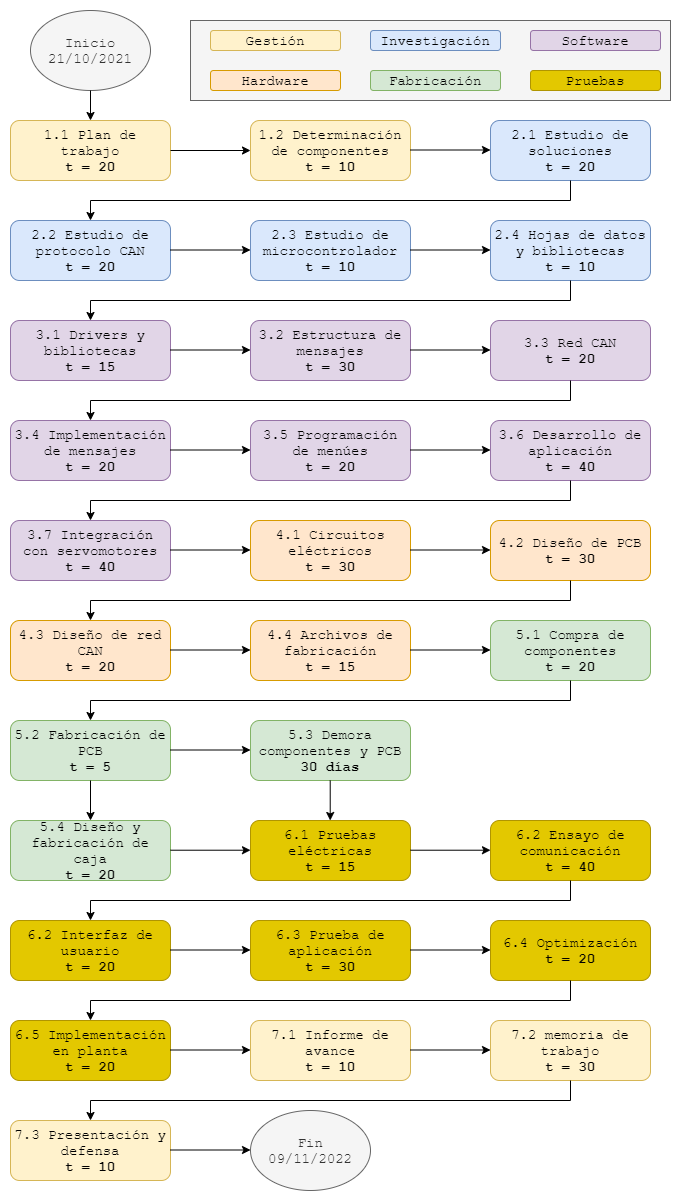
\includegraphics[width=.8\textwidth]{./Figuras/GdP_AoN.png}
\caption{Diagrama en \textit{Activity on Node}}
\label{fig:AoN}
\end{figure}

\section{11. Diagrama de Gantt}
\label{sec:gantt}

En la figura \ref{fig:WBSGantt} se muestra el esquema de desglose de trabajo y en la figura \ref{fig:diagGantt}, el diagrama de gantt del proyecto.

\begin{figure}[htpb]
\centering 
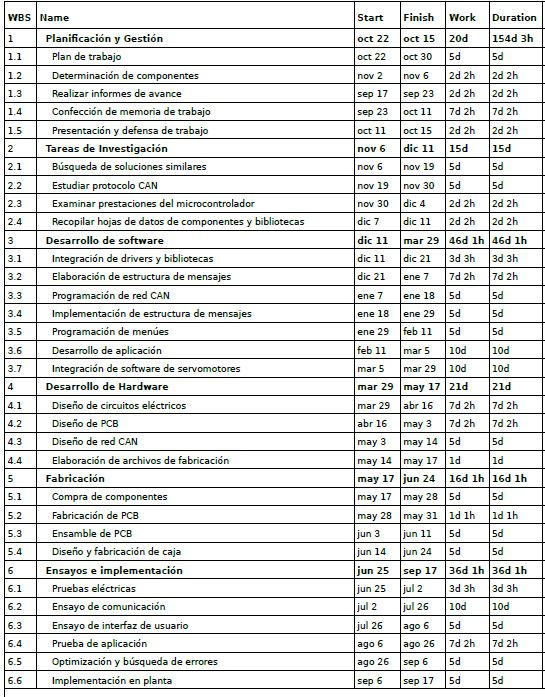
\includegraphics[height=0.7\textheight]{./Figuras/WBS_GdP.JPG}
\caption{Desglose de trabajo}
\label{fig:WBSGantt}
\end{figure}


\begin{figure}[htpb]
\centering 
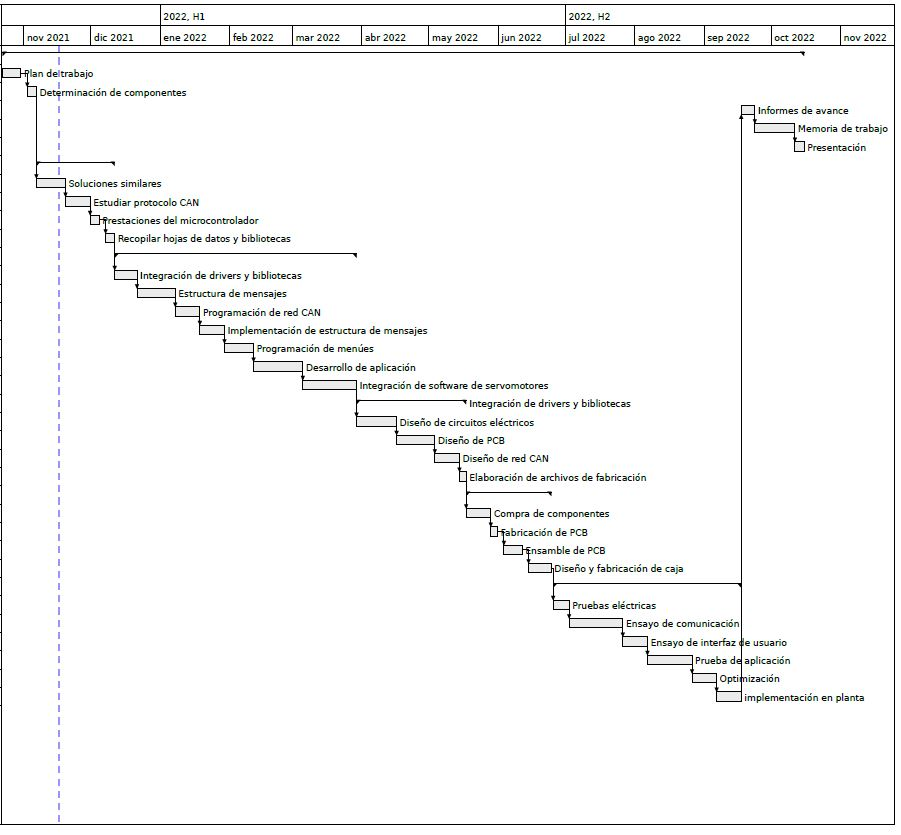
\includegraphics[height=0.65\textheight]{./Figuras/Gantt_GdP.JPG}
\caption{Diagrama de Gantt}
\label{fig:diagGantt}
\end{figure}




\section{12. Presupuesto detallado del proyecto}
\label{sec:presupuesto}

En el cuadro \ref{tab:costosProyecto} se detallan los costos del proyecto.

\begin{table}[htpb]
\centering
\begin{tabularx}{\linewidth}{@{}|X|c|r|r|@{}}
\hline
\rowcolor[HTML]{C0C0C0} 
\multicolumn{4}{|c|}{\cellcolor[HTML]{C0C0C0}COSTOS DIRECTOS} \\ \hline
\rowcolor[HTML]{C0C0C0} 
Descripción &
  \multicolumn{1}{c|}{\cellcolor[HTML]{C0C0C0}Cantidad} &
  \multicolumn{1}{c|}{\cellcolor[HTML]{C0C0C0}Valor unitario} &
  \multicolumn{1}{c|}{\cellcolor[HTML]{C0C0C0}Valor total} \\ \hline
Horas de ingeniería &
  \multicolumn{1}{c|}{630} &
  \multicolumn{1}{c|}{8 U\$} &
  \multicolumn{1}{c|}{5040 U\$} \\ \hline
  
Dispositivos de testing &
  \multicolumn{1}{c|}{1} &
  \multicolumn{1}{c|}{250 U\$} &
  \multicolumn{1}{c|}{250 U\$} \\ \hline
  
Componentes electrónicos &
  \multicolumn{1}{c|}{1} &
  \multicolumn{1}{c|}{300 U\$} &
  \multicolumn{1}{c|}{300 U\$} \\ \hline
  
Placas PCB &
  \multicolumn{1}{c|}{1} &
  \multicolumn{1}{c|}{150 U\$} &
  \multicolumn{1}{c|}{150 U\$} \\ \hline  
  
Servomotores &
  \multicolumn{1}{c|}{4} &
  \multicolumn{1}{c|}{100 U\$} &
  \multicolumn{1}{c|}{400 U\$} \\ \hline  

Fabricación de caja &
  \multicolumn{1}{c|}{1} &
  \multicolumn{1}{c|}{50 U\$} &
  \multicolumn{1}{c|}{50 U\$} \\ \hline 

\multicolumn{3}{|c|}{SUBTOTAL} &
  \multicolumn{1}{c|}{6190 U\$} \\ \hline
\rowcolor[HTML]{C0C0C0} 
\multicolumn{4}{|c|}{\cellcolor[HTML]{C0C0C0}COSTOS INDIRECTOS} \\ \hline
\rowcolor[HTML]{C0C0C0} 
Descripción &
  \multicolumn{1}{c|}{\cellcolor[HTML]{C0C0C0}Cantidad} &
  \multicolumn{1}{c|}{\cellcolor[HTML]{C0C0C0}Valor unitario} &
  \multicolumn{1}{c|}{\cellcolor[HTML]{C0C0C0}Valor total} \\ \hline
  
Horas de administración &
  \multicolumn{1}{c|}{50} &
  \multicolumn{1}{c|}{5 U\$} &
  \multicolumn{1}{c|}{250 U\$} \\ \hline 

Horas de uso de PC &
  \multicolumn{1}{c|}{680} &
  \multicolumn{1}{c|}{0.5 U\$} &
  \multicolumn{1}{c|}{340 U\$} \\ \hline 
  
Horas de uso de máquinas &
  \multicolumn{1}{c|}{40} &
  \multicolumn{1}{c|}{2 U\$} &
  \multicolumn{1}{c|}{80 U\$} \\ \hline 

\multicolumn{3}{|c|}{SUBTOTAL} &
  \multicolumn{1}{c|}{670 U\$} \\ \hline
\rowcolor[HTML]{C0C0C0}
\multicolumn{3}{|c|}{TOTAL} &
\multicolumn{1}{c|}{6890 U\$}
   \\ \hline
\end{tabularx}%
\caption{Costos del proyecto}
\label{tab:costosProyecto}
\end{table}


\section{13. Gestión de riesgos}
\label{sec:riesgos}

a) Riesgos identificados:

Riesgo 1: No habrá stock de los componentes necesarios.
\begin{itemize}
	\item Severidad (S): 8. Sin los componentes no se podrá ensayar ni finalizar el proyecto.
	\item Probabilidad de ocurrencia (O): 7. Actualmente, existe una escasez general de componentes electrónicos por motivo de la pandemia Covid-19. 
\end{itemize}   

Riesgo 2: El fabricante de PCBs tendrá demoras excesivas o problemas con la fabricación.
\begin{itemize}
	\item Severidad (S): 6. Sin la placa, solo se podrá hacer un prototipo provisorio empleando placas de desarrollo. No podrá completarse el proyecto en tiempo de forma satisfactoria
	\item Ocurrencia (O): 2. Hay varios fabricantes, y con los que se trabajó previamente nunca hubo inconvenientes.
\end{itemize}

Riesgo 3: Se producirá un nuevo cierre general de actividades debido a la actual pandemia de Covid-19.
\begin{itemize}
	\item Severidad (S): 8. El cierre impediría la obtención de componentes en tiempo, así como la posibilidad de realizar testeos e implementaciones.
	\item Ocurrencia (O): 4. La situación de la pandemia parece haberse estabilizado en los últimos meses.
\end{itemize}

Riesgo 4: Se perderá la relación actual con la empresa Cambre.
\begin{itemize}
	\item Severidad (S): 5. Se complicaría realizar testeos en planta, así como algunas facilidades para la obtención de los componentes.
	\item Ocurrencia (O): 2. Actualmente, la relación es muy buena.
\end{itemize}

Riesgo 5: Aparecerán trabas políticas en materia aduanera, o complicaciones económicas en Argentina.
\begin{itemize}
	\item Severidad (S): 7. Se dificultaría conseguir los componentes y las PCB.
	\item Ocurrencia (O): 3. Sería muy inusual que ocurriera un cambio tan repentino a nivel político.
\end{itemize}

b) Tabla de gestión de riesgos:      (El RPN se calcula como RPN=SxO)

\begin{table}[htpb]
\centering
\begin{tabular}{|c|c|c|c|c|c|c|}
\hline
\rowcolor[HTML]{C0C0C0} 
Riesgo & Severidad & Ocurrencia & RPN & Severidad* & Ocurrencia* & RPN* \\ \hline
    1  & 8  & 7  &  56   &  6  & 4   & 24     \\ \hline
    2  & 6  & 2  &  12   &  -  &  -  &      \\ \hline
    3  & 8  & 4  &  32   &  6  &  3  & 18     \\ \hline
    4  & 5  & 2  &  10   &  -  &  -  &      \\ \hline
    5  & 7  & 3  &  21   &  -  &  -  &      \\ \hline
\end{tabular}%
\end{table}

Criterio adoptado: 
Se tomarán medidas de mitigación en los riesgos cuyos números de RPN sean mayores a 30.

Nota: los valores marcados con (*) en la tabla corresponden luego de haber aplicado la mitigación.

c) Plan de mitigación de los riesgos que originalmente excedían el RPN máximo establecido:
 
Riesgo 1: Se buscará determinar lo antes posible los componentes a usar y encargarlos de inmediato.
\begin{itemize}
  \item Severidad (S): 6. La severidad es menor ya que el problema se afrontaría antes, permitiendo no atrasarse o seleccionar otros componentes similares y diseñar a partir de estos.
  \item Probabilidad de ocurrencia (O): 4. Si bien puede que no haya stock, se tendrá un mayor margen de tiempo en el cual se pueden conseguir los componentes.
\end{itemize}
  
Riesgo 3: Similar al plan del Riesgo 1, se buscará determinar los componentes lo antes posible y encargarlos.
\begin{itemize}
	\item Severidad (S): 6. Teniendo los componentes en mano, el proyecto tiene menos retrasos debido a un cierre.
  \item Probabilidad de ocurrencia (O): 3. La posibilidad de que ocurra un cierre se mantiene igual, pero la posibilidad de no tener los componentes disminuye.
\end{itemize}


\section{14. Gestión de la calidad}
\label{sec:calidad}

Para cada uno de los requerimientos del proyecto se enuncia el procedimiento de verificación y validación:

\setcounter{REQ}{0}
\begin{itemize} 
	\item \REQ ~El sistema debe comunicarse empleando el protocolo CAN.
	\begin{itemize}
		\item Verificación: Se comprobará en un laboratorio que la señal cumpla lo estipulado por el protocolo.
		\item Validación: Se conectará a un motor y se enviará un mensaje CAN.
	\end{itemize}
	\item \REQ ~El sistema debe poder comunicarse con todos los motores conectados a la red CAN que posean la placa controladora SN-17.
	\begin{itemize}
		\item Verificación: Se verá que el ID del mensaje sea el que corresponde y los filtros y máscaras actúen correctamente.
		\item Validación: Se conectarán varios motores y se enviarán mensajes a cada uno.
	\end{itemize}
	\item \REQ ~El sistema debe poder comunicarse con hasta 5 motores conectados a la red CAN.
	\begin{itemize}
		\item Verificación: Se verá que el ID del mensaje sea el que corresponde y los filtros y mascaras actúen correctamente.
		\item Validación: Se conectarán varios motores y se enviarán mensajes a cada uno.
	\end{itemize}
	\item \REQ ~El sistema debe envíar y recibir información a través del puerto CAN a una tasa de al menos 300 kbps.
	\begin{itemize}
		\item Verificación: Se comprobará en un laboratorio que se cumplan los tiempos de señal.
		\item Validación: Se conectará un motor y se enviarán mensajes a la tasa estipulada.
	\end{itemize}
	\item \REQ ~El sistema debe poder enviar programas a los servomotores de hasta 15 instrucciones de largo.
	\begin{itemize}
		\item Verificación: Se verá que el mensaje pueda indicar correctamente el número de instrucción con 4 bits.
		\item Validación: Se enviará a un motor un programa con 15 instrucciones.
	\end{itemize}
	\item \REQ ~El sistema debe tener la capacidad de enviar cada una de las instrucciones de programa disponibles en los servomotores. Estas son: Seteo de tipo de control, verificación de señal de control, pausa de la señal de control, apagado de control, comunicación, reseteo de programa.
	\begin{itemize}
		\item Verificación: Se verá que el mensaje pueda indicar correctamente la instrucción.
		\item Validación: Se enviará a un motor cada una de las instrucciones.
	\end{itemize}
	\item \REQ ~El sistema debe enviar, para cada instrucción, todos los atributos de configuración necesarios. Estos son: Selección de variable de control, seteo de variable de control, tiempo de cumplimiento de instrucción, tiempo de timeout, error permisible de la variable de control, torque máximo de motor, tipo de comunicación y mensaje.
	\begin{itemize}
		\item Verificación: Se verá que el mensaje pueda indicar correctamente la instrucción.
		\item Validación: Se enviará a un motor cada una de las instrucciones.
	\end{itemize}
	\item \REQ ~El sistema debe poder modificar los parámetros de los lazos de control PID de los servomotores para los distintos tipos de control.
	\begin{itemize}
		\item Verificación: Se verá que el mensaje pueda indicar correctamente la configuración.
		\item Validación: Se enviará a un motor cada una de las configuraciones.
	\end{itemize}
	\item \REQ ~El sistema debe poder configurar el seteo de funcionalidades especiales de los motores, estas son: selección de tipo de cerado (\textit{homing}), proceso de cerado, calibración del encoder, calibración de posiciones, forma de operatividad de las salidas discretas de los motores, verificación de detención de eje.
	\begin{itemize}
		\item Verificación: Se verá que el mensaje pueda indicar correctamente la funcionalidad.
		\item Validación: Se enviará a un motor cada una de las funcionalidades.
	\end{itemize}
	\item \REQ ~El sistema debe permitir operar los motores en forma manual, simulando las entradas y forzando las salidas discretas que cada uno de los motores conectados.
	\begin{itemize}
		\item Verificación: Se verá que el mensaje pueda indicar correctamente la IO a operar.
		\item Validación: Se enviará a un motor cada una de las IO.
	\end{itemize}
	\item \REQ ~El sistema deberá poder activar o desactivar a cada uno de los motores conectados.
	\begin{itemize}
		\item Verificación: Se verá que el mensaje pueda indicar correctamente el motor a activar/desactivar.
		\item Validación: Se enviará a varios motores conectados una señal de activado y desactivado.
	\end{itemize}
	\item \REQ ~El sistema deberá recibir de cada motor conectado el número de programa e instruccion en que se encuentra.
	\begin{itemize}
		\item Verificación: Se verá que el mensaje pueda indicar el número de programa e instrucción
		\item Validación: Se conectará un motor en funcionamiento y se comprobará el estado de este a través de la pantalla.
	\end{itemize}
	\item \REQ ~El sistema deberá recibir de cada motor conectado un reporte de error en caso de falla.
	\begin{itemize}
		\item Verificación: Se verá que el mensaje pueda indicar correctamente el error.
		\item Validación: Se conectará un motor en funcionamiento y se comprobará el estado de error a través de la pantalla.
	\end{itemize}
	\item \REQ ~El sistema debe poder comunicarse con un controlador externo (PLC) a través de señales discretas.
	\begin{itemize}
		\item Verificación: Se verá en un laboratorio que el sistema pueda recibir y enviar señales discretas.
		\item Validación: Se conectará un PLC que enviará señales discretas y se comprobará el funcionamiento a través de la pantalla.
	\end{itemize}
	\item \REQ ~Las señales al controlador externo deben estar eléctricamente aisladas, por lo menos a 1 kV, usando optoacopladores.
	\begin{itemize}
		\item Verificación: Se verá el datasheet de los optoacopladores empleados y se comprobaran las distancias de aislación eléctrica en la PCB.
		\item Validación: Se hará un ensayo de sobretensión en el sistema.
	\end{itemize}
	\item \REQ ~Las señales al controlador externo deben ser del tipo NPN.
	\begin{itemize}
		\item Verificación: Se comprobarán los esquemáticos de los PCB y los componentes seleccionados.
		\item Validación: Se hará una demostración con instrumentos de medición de tipo de salida.
	\end{itemize}
	\item \REQ ~Las señales al controlador externo deben poder ser a distinta tensión que la empleada por el microcontrolador, hasta 24V.
	\begin{itemize}
		\item Verificación: Se comprobarán los esquemáticos de los PCB y los componentes seleccionados.
		\item Validación: Se conectará un PLC que trabaje a 24V y se enviarán señales que comprueben el funcionamiento.
	\end{itemize}
	\item \REQ ~El sistema deberá enviar señales discretas en caso de que alguno de los motores conectados reporte un error.
	\begin{itemize}
		\item Verificación: Se verá en el código que se cumpla la funcionalidad requerida.
		\item Validación: Se conectará un motor y un PLC y se forzará una situación de error.
	\end{itemize}
	\item \REQ ~El sistema debe tener una pantalla LCD y una botonera.
	\begin{itemize}
		\item Verificación: Se comprobarán los componentes empleados.
		\item Validación: Se comprobará la conformación del sistema.
	\end{itemize}
	\item \REQ ~La pantalla LCD debe permitir acceder a las variables de los motores a través de un menú y debe recorrerse usando la botonera. 
	\begin{itemize}
		\item Verificación: Se comprobará el codigo del sistema.
		\item Validación: Se realizará una prueba de funcionamiento.
	\end{itemize}
	\item \REQ ~El sistema debe tener un switch que permita cambiar su forma de funcionamiento, entre configurador de motores y relevador de información.
	\begin{itemize}
		\item Verificación: Se comprobará el codigo del sistema.
		\item Validación: Se realizará una prueba de funcionamiento.
	\end{itemize}
	\item \REQ ~El sistema debe emplear el microcontrolador ATSAMC21.
	\begin{itemize}
		\item Verificación: Se comprobará el uso del componente.
		\item Validación: Se comprobará el uso del componente.
	\end{itemize}
	\item \REQ ~El sistema debe alimentarse con 24V de tensión.
	\begin{itemize}
		\item Verificación: Se comprobarán los esquemáticos y los componentes elegidos.
		\item Validación: Se conectará el sistema a 24V y se verá su funcionamiento.
	\end{itemize}
	\item \REQ ~El sistema debe estar encapsulado dentro de una caja plástica.
	\begin{itemize}
		\item Verificación: Se comprobarán los dibujos y planos mecánicos del sistema.
		\item Validación: Se verá la presentación del sistema.
	\end{itemize}
\end{itemize}
		
\section{15. Procesos de cierre}    
\label{sec:cierre}

A continuación se enuncian cuáles serán las actividades de cierre del proyecto y quien será el encargado de su organización:

\begin{itemize}
	\item Reunión de evaluación de proyecto: A realizar con \supname , director del trabajo. Se estudiará en que medida se respetó el plan de proyecto original, comparando con los resultados obtenidos. También se evaluarán las técnicas emlpeadas y se las distinguirá entre eficientes e ineficientes, según si ayudaron a que el proyecto se realice en tiempo y cumpliendo las pautas de calidad y riesgo. Se escribirá un documento que detalle las conclusiones de dicha reunión, como referencia para proyectos futuros. (Encargado: \authorname) 
	\item Reunión de agradecimiento: A realizar con \supname , director del trabajo y los colaboradores de Cambre, que ayuden en la implementación en planta. (Encargado: \authorname)
\end{itemize}


\end{document}
